% !TeX spellcheck = en_US
\documentclass[12pt, a4paper]{report}
\usepackage[scaled]{helvet}
\renewcommand\familydefault{\sfdefault}
\usepackage[T1]{fontenc}
\usepackage[margin=0.5in]{geometry}
\usepackage{float}
\usepackage{framed}
\usepackage{multicol}
\usepackage{amsmath}
\usepackage{amssymb}
\usepackage[framemethod=TikZ]{mdframed}
\usepackage{graphicx}
\usepackage{enumitem}
\usepackage{gensymb}
\setlist{nosep}
\usepackage{booktabs}
\usepackage{makecell}
\usepackage{tikzsymbols}
\usepackage{hyperref}
\hypersetup{
	colorlinks,
	citecolor=black,
	filecolor=black,
	linkcolor=black,
	urlcolor=black
}
\usepackage{multirow}
\usepackage{pgf-umlsd}
\usepackage{soul}
\usepackage{pgfplots}
\usepackage{tikz}
\tikzstyle{dot} = [shape=circle, fill=black]
%\usepgfplotslibrary{external}
%\tikzexternalize

\newcounter{note}\setcounter{note}{0}
\renewcommand{\thenote}{\arabic{note}}
\newenvironment{note}[1]{
	\stepcounter{note}
	\ifstrempty{#1}{
		\mdfsetup{
			frametitle={
				\tikz[baseline=(current bounding box.east),outer sep=0pt]
				\node[anchor=east,rectangle,fill=blue!20]
				{\strut Note~\thenote};
			}
		}
	}{
		\mdfsetup{
			frametitle={
				\tikz[baseline=(current bounding box.east),outer sep=0pt]
				\node[anchor=east,rectangle,fill=blue!20]
				{\strut Note~\thenote:~#1};
			}
		}
	}
	\mdfsetup{innertopmargin=0pt,linecolor=blue!20,linewidth=2pt,topline=true,frametitleaboveskip=\dimexpr-\ht\strutbox\relax}
	\begin{mdframed}[]\relax
}{
	\end{mdframed}
}
\newenvironment{code}{\ttfamily}{\par}

\begin{document}
	\tableofcontents
	\vspace{2em}
	\textbf{Contributors:}
	\begin{itemize}
		\item Daniel Fitz (Sanchez)
	\end{itemize}
	\newpage

\begin{multicols*}{2}

\chapter{Lecture Notes}
% !TeX spellcheck = en_US
% !TeX root = notes.tex
\section{Thinking Like an Economist}
\subsection{What is Economics?}
\begin{leftbar}
	\noindent\textbf{Life} is about making choices.\\
	Economics is the \textbf{science of} choice.\\
	That means economics is the \textbf{science of life.}
\end{leftbar}
by Mr. Alan Duhs (Senior Lecturer, UQ School of Economics
\subsubsection{What is Microeconomics?}
\begin{itemize}
	\item How to use what you have (your resources) to get as much as possible of what you want
	\item It's mostly about how individuals make the most efficient (effective) choices
	\item The systematic effects these choices have on other individuals
\end{itemize}

\begin{note}{Scarcity Principle}
	Our resources are limited, so getting more of one thing means getting less of another.
	\begin{itemize}
		\item Wants exceeds available resources
		\item Choices between alternatives needed
	\end{itemize}
	Something is \textbf{scarce} if you:
	\begin{itemize}
		\item have to sacrifice something else to get it (e.g. money, time, effort)
		\item need to pay a price for it (i.e. not free)
	\end{itemize}
	\begin{description}
		\item[Consumers] will be forced to decide what to consume
		\item[Producers] will be forced to decide what to produce
		\item[Governments] will be forced to decide how to allocate resources to achieve specified objectives
	\end{description}
\end{note}

\subsection{Opportunity Cost}
All about what was \textbf{not} chosen. Economic concept to help make a rational choice. What was sacrificed. What is given up once a decision has been made.

\subsection{Cost Benefit Principle}
Chose to do something only if the \textbf{extra benefit} (incremental benefit) from doing it is greater than (or equal to) the \textbf{extra cost} (incremental cost), assuming the individual is \textbf{rational}.

\subsection{Economic Surplus}
Incremental benefits of an action minus the incremental explicit and implicit costs of that action
\begin{description}
	\item[Explicit cost] a cost that involves spending money (i.e. a transaction physically occurs)
	\item[Implicit cost] a non-monetary \textbf{``opportunity cost''} (no transaction occurs but an alternative is not chosen)
\end{description}
Econmic decision strive to maximize economic surplus by:
\begin{enumerate}
	\item \textbf{maximizing} the benefits
	\item \textbf{minimizing} the costs
\end{enumerate}
Economic surplus can be maximized by making choices that \textbf{minimize the opportunity cost}. \textbf{Opportunity cost} is economics is about assessing if an \textbf{efficient choice} of resources has been made.

\subsection{Rules for Making Rational Economic Choices}
In economics, a rational choice should:
\begin{enumerate}
	\item \textbf{include} opportunity cost
	\item \textbf{exclude} sunk cost
	\item measure cost in \textbf{absolute dollar amount}, not percentages
	\item be based on \textbf{Marginal Analysis}
\end{enumerate}

\begin{note}{Sunk Cost}
	\begin{itemize}
		\item expenses that have occurred in the past before a decision has been taken
		\item costs that would have had to occur in order for a choice to be made
		\item costs that are typically not able to be directly recovered
		\begin{enumerate}
			\item exploration costs (oil well, mining)
			\item market research costs (focus groups, surveys)
			\item feasibility study costs (before a decision is made)
		\end{enumerate}
	\end{itemize}
\end{note}

\subsection{Marginal Benefit}
The change in total benefit from doing \textbf{one extra unit of} an activity
$$ = \frac{\text{change in total benefit}}{\text{one extra unit sold}}$$
\subsection{Marginal Cost}
The change in total cost from doing \textbf{one extra unit of} an activity
$$ = \frac{\text{change in total cost}}{\text{one extra unit produced}}$$

\begin{note}{Economic Efficiency}

\end{note}
% !TeX spellcheck = en_US
% !TeX root = notes.tex
%\section{Thinking Like An Economist 2}
\subsection{Absolute and Comparative Advantage}
\subsubsection{Absolute Advantage}
\begin{itemize}
	\item ability of an individual, firm, or country \textbf{to produce more} of a product or service than competitors using the \textbf{same amount} of resources.
	\item alternatively, produce the \textbf{same} amount of product or services as competitors with \textit{less resources}.
\end{itemize}
\subsubsection{Comparative Advantage}
\begin{itemize}
	\item ability of an individual, firm, or country to produce a product or service at a \textit{lower opportunity cost} than other competitors (relates to who is more efficient at producing something).
\end{itemize}
Opportunity cost is about assessing if an \textbf{efficient choice} of resources has been made. Outcomes are efficient if opportunity cost is minimised. \textbf{Comparative advantage} exists with the producer (or service provider) producing the product at the \textbf{lowest opportunity cost}. Contrast \textbf{absolute advantage} which is \textit{irrelevant} in deciding who is more efficient at producing something.

\subsection{Gains and Specialization}
\begin{note}{Principle of Comparative Advantage}
	\begin{itemize}
		\item Everyone does best (individuals or countries) when they concentrate on activities for which their opportunity cost is lowest.
		\item By exchanging goods with others, individuals can more efficiently obtained their preferred mix of goods and services.
	\end{itemize}
\end{note}

\subsection{Production Possibility Curve (PPC)}
\begin{itemize}
	\item The production possibilities curve (PPC) = a graphical representation describing the maximum amount of one good that can be produced for every possible level of production of another good.
	\item\textbf{Assumptions:}
	\begin{enumerate}
		\item only two goods are able to be produced (for simplification), bananas and blueberries
		\item consider the PPC for a single worker only
	\end{enumerate}
\end{itemize}
\begin{description}
	\item[Attainable Point:] Any combination of goods that can be produced using currently available resources. All points on the PPC, as well as below and to the left of the PPC, are attainable.
	\item[Unattainable Point:] Any combination of goods that cannot be produced using currently available resources. All points lying above and to the right of the PPC are unattainable.
	\item[Efficient Point:] Any combination of goods for which currently available resources \textbf{do not} allow an increase in the production of one good unless there is a reduction in the production of the other.
	\item[Inefficient Point:] Any combination of goods for which currently available resources \textbf{enable} an increase in the production of one good \textbf{without} a reduction in the production of the other.
\end{description}
% !TeX spellcheck = en_US
% !TeX root = notes.tex
\section{Binary Arithmetic}
\subsection{Equivalent Circuits}
All circuits can be constructed from NAND and NOR gates

\subsection{Overflow}
Overflow with two's complement addition:
\begin{itemize}
	\item Carry into sign-bit is different to the carry out of the sign-bit
	\item Equivalently, overflow occurs if
	\subitem Two negatives added together give a positive, or
	\subitem Two positives added together give a negative	
\end{itemize}

\subsection{Full Adder}
\begin{figure}[H]
	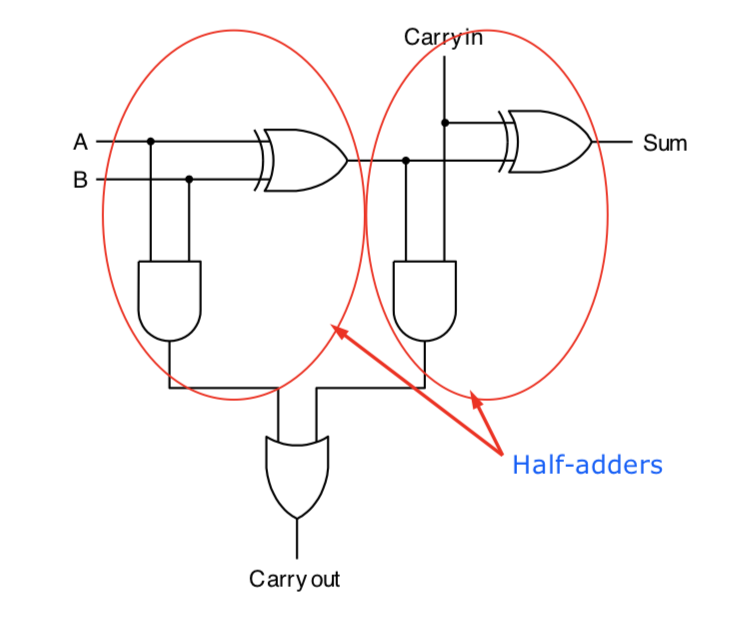
\includegraphics[width=0.8\linewidth]{fulladder}	
\end{figure}


\subsection{Binary Adder}
Can cascade full adders to make binary adder. This is a \textbf{ripple-carry adder}.
\begin{figure}[H]
	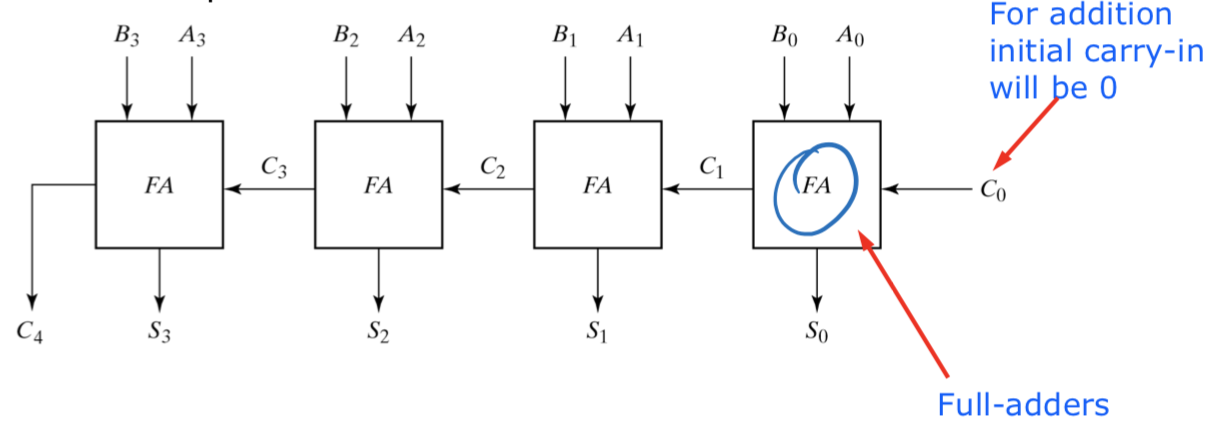
\includegraphics[width=0.8\linewidth]{binaryadder}	
\end{figure}



%\begin{circuitikz}
%	\draw (1, -2) node [and port,rotate=-90] (and1) {};
%	\draw (5, -2) node [and port,rotate=-90] (and2) {};
%	\draw (3, -4) node [or port,rotate=-90] (or1) {};
%	\draw (and1.out) |- (or1.in 2);
%	\draw (and2.out) |- (or1.in 1);
%	
%	\draw (3, 0.5) node [xor port] (xor1) {};
%	
%	\draw (0, 0) node (a) {A};
%	\draw (0, 1) node (b) {B};
%	
%	\draw (a) -| (and1.in 1);
%	\draw (a) -| (xor1.in 2);
%	\draw (b) -| (and1.in 2);
%	\draw (b) -| (xor1.in 1);
%\end{circuitikz}

% !TeX spellcheck = en_US
% !TeX root = notes.tex
\section{Combination Logic}
\subsection{Combinational Circuits}
Each output can be expressed as a function of $n$ input variables. Can write truth table also:
\begin{itemize}
	\item $n$ input columns
	\item $m$ output columns
	\item $2^n$ rows (i.e. possible input combination)
\end{itemize}

\begin{note}{Multiplexer (or Mux)}
	\begin{itemize}
		\item $2^n$ data inputs
		\item 1 output
		\item $n$ control (or \textbf{select}) inputs - that \textbf{select} one of the inputs to be ``sent'' or ``steered'' to the output	
	\end{itemize}
\end{note}

\begin{note}{Decoder}
	Converts $n$-bit input to a logic-1 on exactly one of $2^n$ outputs	
\end{note}

\subsection{Timing Diagram}
\begin{figure}[H]
	\begin{tikztimingtable}[timing/slope=0,timing/coldist=2pt,xscale=4,semithick]
		Input & LHL \\
		Output & HLH \\
		\extracode\makeatletter
		\begin{pgfonlayer}{background}
			\begin{scope}[gray,semitransparent,semithick]
				\horlines{}
				\vertlines{0,...,3}	
			\end{scope}
		\end{pgfonlayer}
	\end{tikztimingtable}
	\centering\caption{Timing Diagram of an inverter}
\end{figure}

There is a slight delay in logic timings in reality
\begin{figure}[H]
	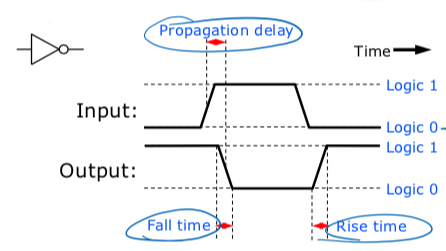
\includegraphics[width=0.8\linewidth]{timing}
	\centering\caption{Reality of Timing}
\end{figure}
\begin{description}
	\item[Propagation delay:] time for change in input to affect output
	\item[Fall time:] time taken for output to fall from 1 to 0
	\item[Rise time:] time for output to rise from 0 to 1	
\end{description}





%\end{multicols*}

\chapter{EMC Tutes}
% !TeX spellcheck = en_US
% !TeX root = notes.tex
\section{Supply and Demand}
\begin{figure}[H]
	\centering
	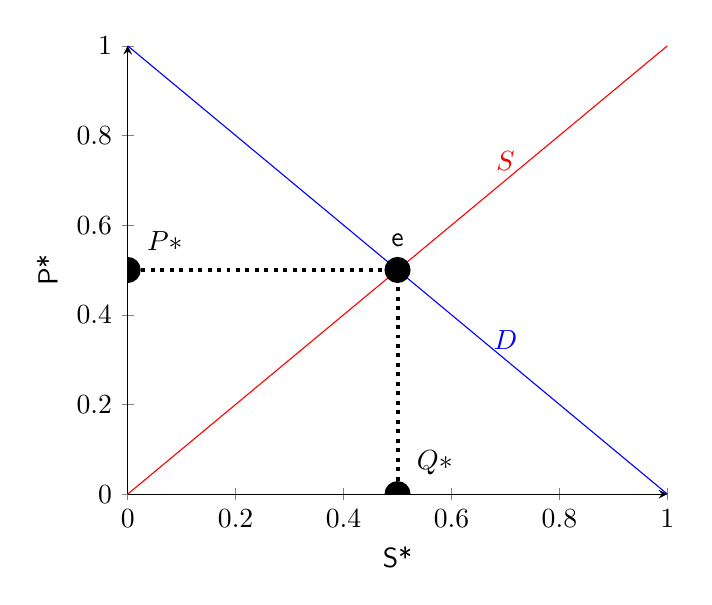
\begin{tikzpicture}
		\begin{axis}[axis lines=left,xlabel={S*},ylabel={P*}]
			\addplot[domain=0:1,color=blue]{1-x} node[above,pos=0.7] {$D$};
			\addplot[domain=0:1,color=red]{x} node[above,pos=0.7] {$S$};
			\node[label={e},dot] (e) at (axis cs:0.5,0.5){};
			\node[label={45:{$P*$}},dot] (p) at (axis cs:0,0.5){};
			\node[label={45:{$Q*$}},dot] (q) at (axis cs:0.5,0){};
			\draw[dotted, line width=0.5mm] (p) -- (e);
			\draw[dotted, line width=0.5mm] (q) -- (e);
		%	\node[dot] (left) at (axis cs:8,2){};
		%	\node[dot] (right) at (axis cs:16,2){};
		%	\draw[->, line width=0.7mm] (right) -- (left);
		%	\draw[dotted, line width=0.5mm] (axis cs:0,2) -- (left);
		%	\draw[dotted, line width=0.5mm] (axis cs:8,0) -- (left);
		%	\draw[dotted, line width=0.5mm] (axis cs:16,0) -- (right);
		\end{axis}
	\end{tikzpicture}
	\caption{Left Shift in demand}\label{fig:left}
\end{figure}
% !TeX spellcheck = en_US
% !TeX root = notes.tex
\section{Perfect Competition}
\begin{itemize}
	\item Free entry and exist
	\item Homogeneous Product
	\item Mark clear at equilibrium
	\item Perfect information
	\item Large number of buyers and sellers
	\item Firms of price taker
\end{itemize}

\section{Market Equilibrium}
A Demand Curve is downward sloping because people are more likely to be excited about buying something when it is cheap.


\end{multicols*}

\chapter{CML Quizzes}
% !TeX spellcheck = en_US
% !TeX root = notes.tex
\section{Quiz 1}

\subsection{Question 1}
Rosie is considering starting a clothing stall at a weekend market in her suburb. Which of the following statements is true? (Single Answer)
\begin{enumerate}
	\item \hl{Rosie can use economic thinking to determine the selling price of her cloths}
	\item Rosie should only use economics in this situation and not accounting
	\item Clothing is not a scarce resource
	\item Rosie cannot use economics because her business is too small
	\item Rosie does not have to make trade-offs in this situation
\end{enumerate}

\subsection{Question 2}
Andy is a baker in Brisbane. It costs him \$0.50 to produce each loaf of bread. Andy can sell 10 loaves of bread for \$40 and 11 loaves of bread for \$43. Which of the following statements are true: (Multiple Answers)
\begin{enumerate}
	\item \hl{The marginal cost of producing a loaf of bread is \$0.50}
	\item \hl{Andy should produce the eleventh loaf of bread because marginal benefit is greater than the average cost}
	\item There is insufficient information to determine the marginal benefit of producing the eleventh loaf of bread
	\item \hl{The marginal benefit of producing the eleventh loaf of bread is \$3}
\end{enumerate}\vspace{1em}
Working:
\begin{table}[H]
	\centering
	\begin{tabular}{r|rr}
		Number of Loaves & Money Gained & Total Benefit\\\hline
		10 & \$40 & \$35\\
		11 & \$43 & \$37.5\\
	\end{tabular}
\end{table}
\noindent Average cost: \$0.50\\
Marginal Benefit of 11th bread: \$3

\subsection{Question 3}
Jeremy is considering whether to go to the beach on the weekend. His alternatives, in order of preference from most to least preferred, are:
\begin{enumerate}
	\item Visiting his family
	\item Studying for a test
	\item Working at his casual job for 5 hours with a wage of \$15/hour
\end{enumerate}
Select the item from the list provided to make the following statements true:\\\\
Average Cost; The net benefit of working at his casual job; should not; visiting his family; 5 hours; working at his casual job; should; studying for a test; the net benefit of studying for a test; marginal benefit; marginal cost; \$15/hour.\\\\
In considering whether to go to the beach, the value of casual work foregone \_\_\_\_\_\_\_\_\_\_ be included in a marginal analysis. The opportunity cost of going to the beach is \_\_\_\_\_\_\_\_\_\_. If going to the beach suddenly is \textbf{not} an option for Jeremy, then \_\_\_\_\_\_\_\_\_\_ is the opportunity cost of visiting his family.\\\\
Answer: Should not; visiting his family; studying for a test

\subsection{Question 4}
Lillian bought a limited edition ``Harry Potter'' costume at an exclusive fan event. She can now either:
\begin{enumerate}
	\item Sell the costume on eBay for \$534
	\item Keep the costume for per personal use
\end{enumerate}
If she sells the costume on eBay she will have to pay \$10 to ship it to the customer. If she keeps the costume she expects to gain \$651 of enjoyment and will need to spend \$88 on maintenance and cleaning. When comparing the net benefits of selling the costume minus the net benefits of keeping it, what is the economic surplus/loss? Answer to the nearest whole number.\\\\
Answer:
Let $x$ be the benefit of selling. Let $y$ be the benefit of keeping. Let $t$ be the economic surplus/loss of selling minus keeping
\begin{align*}
	x &= \$534 - \$10\\
	&= \$524\\
	y &= \$651 - \$88\\
	&= \$563\\
	t &= x - y\\
	&= \$524 - \$563\\
	&= -\$39
\end{align*}

\subsection{Question 5}
Lucy pays \$40 to enter a theme park. When inside the park, Lucy considers how many rides she should have on the ``Big Drop''. She expects to gain an incremental benefit of \$25 of enjoyment from the first ride, then gain subsequent incremental benefits of \$20 from the second, \$15 from the third, \$10 from the fourth and \$5 from the fifth. The cost of each ride is \$15.\\\\
In determining how many rides to have, the entry free is a/an \_\_\_\_\_\_\_\_\_\_ cost. Using marginal analysis, Lucy should have how many rides? \_\_\_\_\_\_\_\_\_\_. The maximum surplus for Lucy, from doing the number of rides you found in part b, is \$\_\_\_\_\_\_\_\_\_\_. Answer to nearest whole number.\\\\
\begin{table}[H]
	\centering
	\begin{tabular}{rrr}
		Ride No & Benefit & Benefit - Cost\\\hline
		1 & \$25 & \$10\\
		2 & \$20 & \$5\\
		3 & \$15 & \$0\\
		4 & \$10 & -\$5\\
		5 & \$5 & -\$10
	\end{tabular}
\end{table}
Answer: Opportunity Cost; 2 rides; \$15

\subsection{Question 6}
Seth and Ryan are roommates, living together in a house. Both roommates are currently considering who should cook dinner and who should clean up afterwards. Ryan was a trainee chef and a skilled cook. Seth, on the other hand, had previously only lived at home, where his mum cooked everything for him. However, Seth had become very efficient at cleaning up after meals and packing things away. Which of the following is true: (Multiple Answers)
\begin{enumerate}
	\item Seth has a comparative advantage in cooking dinner
	\item \hl{Thinking like an economist in this situation, the roommates should specialise with Ryan cooking and Seth cleaning}
	\item \hl{Ryan has a lower opportunity cost for cooking dinner}
\end{enumerate}

\subsection{Question 7}
Lily and May operate a store that sells fresh juices. There are two main activities: cutting the fruit and juicing the fruit. Lily and May are deciding who should cut and who should juice in order to maximize output.
\begin{table}[H]
	\centering
	\begin{tabular}{r|c|c}
		& Cutting (kg/hr) & Juicing (kg/hr)\\\Xhline{1pt}
		Lily & 3 & 5\\\hline
		May & 2 & 8
	\end{tabular}
\end{table}
Which of the following statements are true: (Multiple Answers)
\begin{enumerate}
	\item For Lily, the opportunity cost of 1kg of cutting is 1.2kg of juicing
	\item \hl{For May, the opportunity cost of 1kg of juicing is 0.25kg of cutting}
	\item May should specialize in cutting
	\item Lily has an absolute advantage in juicing
\end{enumerate}
\begin{table}[H]
	\centering
	\begin{tabular}{r|c|c}
		& Cutting (kg/hr) & Juicing (kg/hr)\\\Xhline{1pt}
		Lily & $\frac{3}{3}=1$ & $\frac{5}{3}=1.67$\\\hline
		May & $\frac{2}{2}=1$ & $\frac{8}{2}=4$
	\end{tabular}
\end{table}
\begin{table}[H]
	\centering
	\begin{tabular}{r|c|c}
		& Cutting (kg/hr) & Juicing (kg/hr)\\\Xhline{1pt}
		Lily & $\frac{3}{5}=0.6$ & $\frac{5}{5}=1$\\\hline
		May & $\frac{2}{8}=0.25$ & $\frac{8}{8}=1$
	\end{tabular}
\end{table}

\subsection{Question 8}
Australia's second biggest tading partner is Japan. Among other things, Australia exports coal to Japan while importing cars. In one trading day, Japan can produce 12 cars per hour and Australia can produce a total of 80 tonnes of coal per hour. Assume cars and coal are the only two things that the two countries trade. Also assume one trading day is 9 hours long.\\
Select the item from the list provided to make the following statements true.\\\\
Cars per hour; 81; Opportunity cost; 720 tonnes of coal; Comparative advantage; 96; Minimized; 108; Cars; Absolute advantage; Tonnes of coal; Maximized\\\\
By specializing, the two countries have minimized \_\_\_\_\_\_\_\_\_\_. In one trading day, Australia will produce \_\_\_\_\_\_\_\_\_\_. In one trading day, Japan will produce \_\_\_\_\_\_\_\_\_\_ cars.\\\\
Answer: Opportunity Cost; 720 tonnes of coal; 108;

\subsection{Question 9}
Lise is hosting a party in 6 hours' time. She wishes to provide guests with her homemade dips -- guacamole and hummus. Shown below is Lisa's production possibilities curve for the next 6 hours.
\begin{figure}[H]
	\centering
	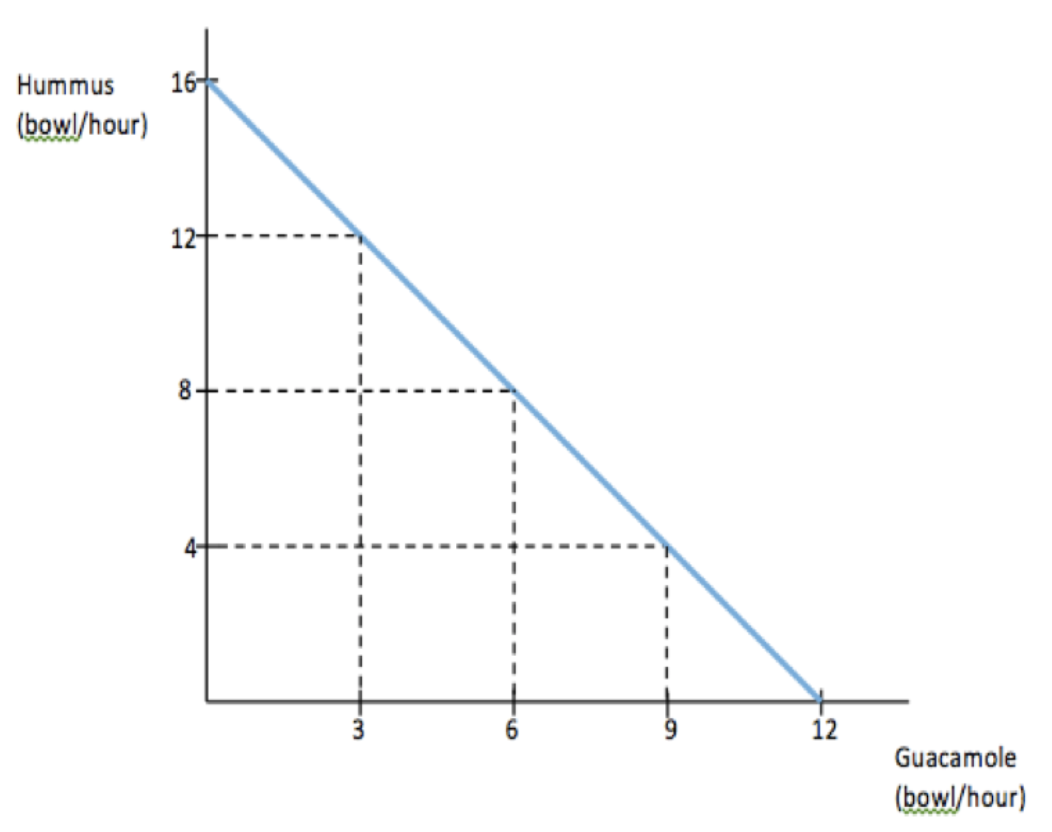
\includegraphics[width=0.5\linewidth]{cml_1_9}
\end{figure}
\noindent What is Lisa's opportunity cost of producing 1 bowl of guacamole? Answer to the nearest two decimal places. In bowls of hummus.\\\\
Answer:
\begin{align*}
	y &= mx+c\\
	16 &= 0m+c\tag{Sub when $x$ is zero}\\
	c &= 16\\
	\therefore y &= mx + 16\\
	0 &= 12m + 16\tag{Sub when $y$ is zero}\\
	-16 &= 12m\\
	m &= \frac{-16}{12} = \frac{-8}{6} = \frac{-4}{3}\\
	\therefore y &= 16 - \frac{4}{3}x\\
	y&= 16 - \frac{4}{3}\times1\tag{Produce 1 bowl of guacamole}\\
	y &= 14.67
\end{align*}
Therefore the opportunity cost of producing 1 bowl of guacamole is $16 - 14.67 = 1.33$ bowls of hummus.

\subsection{Question 10}
Martha is a florist who is trying to maximize her output. She can produce two types of flowers: lilies and violets. Shown below is Martha's production possibilities curve. The X denotes the quantity of each flower she is currently producing.
\begin{figure}[H]
	\centering
	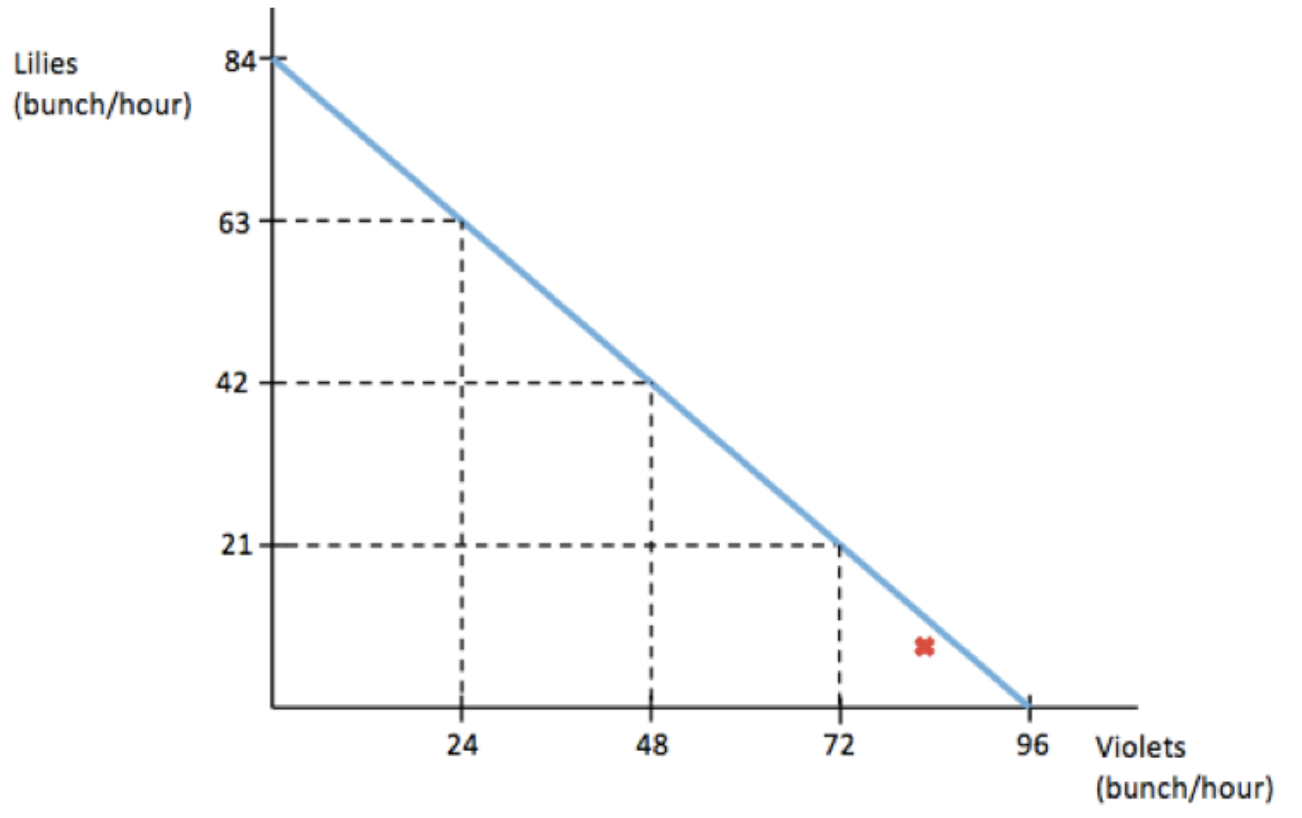
\includegraphics[width=0.5\linewidth]{cml_1_10}
\end{figure}
\noindent Answer the following questions:
\begin{itemize}
	\item Is the current output attainable? (\hl{Yes}/No)
	\item Calculate the opportunity cost of producing 1 bunch of lilies. Answer to the nearest two decimal places. \_\_\_\_\_\_\_\_\_\_ bunches of violets
	\item Is the current output efficient, \hl{inefficient} or neither because it is unattainable?
\end{itemize}\vspace{1em}
\begin{align*}
	y &= 84 - \frac{21}{24}x\\
	1 &= 84 - \frac{21}{24}x\tag{Producing 1 bunch of lillies}\\
	\frac{21}{24}x &= 83\\
	x &= \frac{83\times24}{21}\\
	x &= 94.86
\end{align*}
Therefore the opportunity cost of producing 1 bunch of lilies is $96 - 94.86 = 1.14$
% !TeX spellcheck = en_US
% !TeX root = notes.tex
\section{Quiz 1 Second Attempt}

\subsection{Question 1}
Rosie is considering starting a clothing stall at a weekend market in her suburb. Which of the following statements is true? (Single)
\begin{itemize}
	\item\hl{Rosie can use economic thinking to determine the selling price of her clothes}
	\item Rosie should only use economics in this situation and not accounting
	\item Clothing is not a scarce resource
	\item Rosie cannot use economics because her business is too small
	\item Rosie does not have to make trade-offs in this situation
\end{itemize}

\subsection{Question 2}
John enjoys boxing and engages a personal trainer to improve his health and fitness. As part of a special offer, John pays \$0 for the first session and \$30 for each subsequent session. John gains \$200 of benefit from attending 6 sessions and \$250 of benefit from attending 7 sessions. (Multiple)
\begin{itemize}
	\item\hl{John should attend the seventh session because the marginal benefit is greater than the marginal cost}
	\item The marginal benefit of attending the seventh session is \$40 per session
	\item John should not attend the seventh session because the marginal benefit is less than the marginal cost
	\item The marginal cost of attending the seventh is \$50 per session
\end{itemize}

\subsection{Question 3}
Jeremy is considering whether to go to the beach on the weekend. His alternatives, in order of preference from most to least preferred, are:
\begin{enumerate}
	\item Visiting his family
	\item Studying for a test
	\item Working at his casual job for 5 hours with a wage of \%15/hour
\end{enumerate}
Select the item from the list provided to make the following statements true.
\begin{multicols}{3}
	\begin{itemize}
		\item average cost
		\item the net benefit of working at his casual job
		\item should not
		\item visiting his family
		\item 5 hours
		\item working at his casual job
		\item should
		\item studying for a test
		\item the net benefit of studying for a test
		\item marginal benefit
		\item marginal cost
		\item \$15/hour
	\end{itemize}
\end{multicols}
In considering whether to go to the beach, the value of casual work foregone \_\_\_\_\_\_\_\_\_\_ be included in a marginal analysis.\\
The opportunity cost of going to the beach is \_\_\_\_\_\_\_\_\_\_.\\
If going to the beach suddenly is \textbf{not} an option for Jeremy, then \_\_\_\_\_\_\_\_\_\_ is the opportunity cost of visiting his family.\\\\
Answer: should not; visiting his family; studying for a test

\subsection{Question 4}
Matt is a semi-professional scooter rider and is considering buying a new standard wheel for his scooter. Matt can buy a wheel from the local skate shop on his street for \$30. However, at the skate super store on the other side of town there is a sale of 22\% off for the same wheel . The round trip to the skate super store is 3 hours and therefore Matt must give up 3 hours of sleeping, which he values at a total of \$45. In considering whether Matt should travel to the skate super store to buy the wheel, what is the economic surplus/loss to the nearest whole dollar? Answer to the nearest whole number (with no decimal places or \$ sign. If a loss, include a minus sign).
\begin{align*}
	\text{Discount Cost} &= 30 - 30\times0.22\\ &= 23.4\\
	\text{Total SuperStore Cost} &= 45 + 23.4\\ &= 68.4\\
	\text{Total Loss} &= 68.4 - 30\\ &= 38.4\\ &= 38 \tag{Rounded}
\end{align*}

\subsection{Question 5}
Eloise pays \$20 for a daily pass to the ice skating centre. When inside the centre, Eloise considers how many hours of training she should complete. She expects to gain an incremental benefit of \$57 from the first hour, then gain subsequent incremental benefits of \$40 from the second, \$30 from the third, \$15 from the fourth and \$5 from the fifth. The cost to Eloise, due to the risk of injury and fatigue, is \$4 for the first hour, \$8 for the second hour, \$12 for the third hour, \$16 for the fourth hour and \$20 for the fifth hour.\\\\
In determining how many hours to train for, should the price of the daily pass be included? (Yes/\hl{No})\\
Using marginal analysis, Eloise should train for many hours? \hl{3}\\
The maximum surplus for Eloise, from training the number of hours you found in part b, is....
\[
	(57 + 40 + 30) - (4 + 8 + 12) = 103
\]

\subsection{Question 6}
Drake and Josh work at their local movie theatre. Josh is more efficient at bagging the popcorn, while Drake is more efficient at selling the tickets.\\
Which of the following statements is true? (Single)
\begin{itemize}
	\item \hl{Drake has a lower opportunity cost in selling the tickets}
	\item Josh has a lower opportunity cost in selling the tickets
	\item Josh's absolute advantage is bagging popcorn is relevant in this case when a theatre manager decides who should sell tickets and who bags popcorn
	\item Drake and Josh should not specialise and do both activities themselves for an efficient outcome
	\item The most efficient outcome is where opportunity cost is maximized
\end{itemize}

\subsection{Question 7}
Lily and May operate a store that sells fresh juices. There are two main activities: cutting the fruit and juicing the fruit. Lily and May are deciding who should cut and who should juice in order to maximise output.
\begin{table}[H]
	\centering
	\begin{tabular}{r|cc}
		& Cutting (kg/hr) & Juicing (kg/hr)\\\hline
		Lily & 3 & 5\\
		May & 2 & 8
	\end{tabular}
\end{table}
Which of the following statements are true: (Multiple)
\begin{itemize}
	\item For Lily, the opportunity cost of 1kg of cutting is 1.2kg of juicing
	\item\hl{For May, the opportunity cost of 1kg of juicing is 0.25kg of cutting}
	\item May should specialize in cutting
	\item Lily has an absolute advantage in juicing
\end{itemize}

\subsection{Question 8}
Australia's second biggest trading partner is Japan. Among other things, Australia exports coal to Japan while importing cars. In one trading day, Japan can produce 12 cars per hour and Australia can produce a total of 80 tonnes of coal per hour. Assume cars and coal are the only two things that the two countries trade. Also assume one trading day is 9 hours long.
\begin{multicols}{3}
	\begin{itemize}
		\item Cars per hour
		\item 81
		\item Opportunity cost
		\item 720 tonnes of coal
		\item Comparative advantage
		\item 96
		\item Minimised
		\item 108
		\item Cars
		\item Absolute advantage
		\item Tonnes of coal
		\item Maximised
	\end{itemize}
\end{multicols}
By specialising, the two countries have minimised \_\_\_\_\_\_\_\_\_\_.\\
In one trading day, Australia will produce \_\_\_\_\_\_\_\_\_\_.\\
In one trading day, Japan will produce \_\_\_\_\_\_\_\_\_\_ cars.\\\\
Answers: Opportunity cost; 720 tonnes of coal; 108

\subsection{Question 9}
Roy owns a vineyard and is considering what to produce with his grapes. He can either produce red wine or grape juice (both measured in litres). Shown below is Roy's production possibilities curve for his farm which is 250 square metres.
\begin{figure}[H]
	\centering
	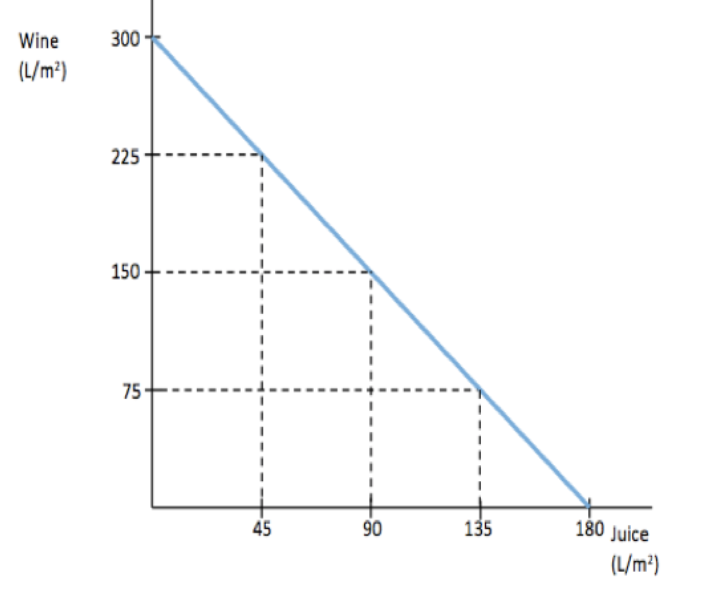
\includegraphics[width=0.6\linewidth]{cml_1_2_9}
\end{figure}
What is his opportunity cost of producing 1 litre of grape juice? Answer to the nearest two decimal places. [a] litres of wine.
\begin{align*}
	y &= 300 - \frac{75}{45}x\\
	&= 300 - \frac{75}{45}\\
	&= 298.33
\end{align*}
Therefore the opportunity cost is $300 - 298.33 = 1.67$

\subsection{Question 10}
Hilary owns a bakery and is trying to decide how to maximise her output. The two baked goods she sells are brownies and muffins. Shown below is Hilary's production possibilities curve. The X denotes the quantity of brownies and muffins she currently produces.
\begin{figure}[H]
	\centering
	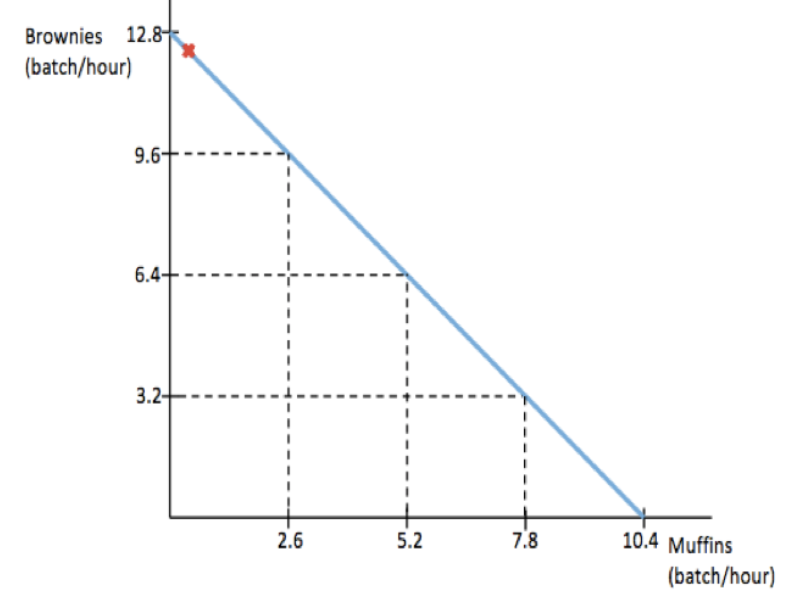
\includegraphics[width=0.6\linewidth]{cml_1_2_10}
\end{figure}
\noindent Is the current output attainable? (\hl{Yes}/No)\\
Is the current output \hl{efficient}, inefficient, or neither because it is unattainable?
Calculate the opportunity cost of producing 1 batch of muffins.
\begin{align*}
	y &= 12.8 - \frac{3.2}{2.6}x\\
	&= 12.8 - \frac{3.2}{2.6}\\
	&= 11.57
\end{align*}
Therefore the opportunity cost is $12.8 - 11.57 = 1.23$

%\end{multicols*}
\end{document}
